\section{Supervised Learning}
\begin{itemize}
	\item The perspective on supervised learning in this course is summarized in Figure~\ref{fig:chapter_6_supervised_learning}
	\begin{figure}[ht!]
		\centering
		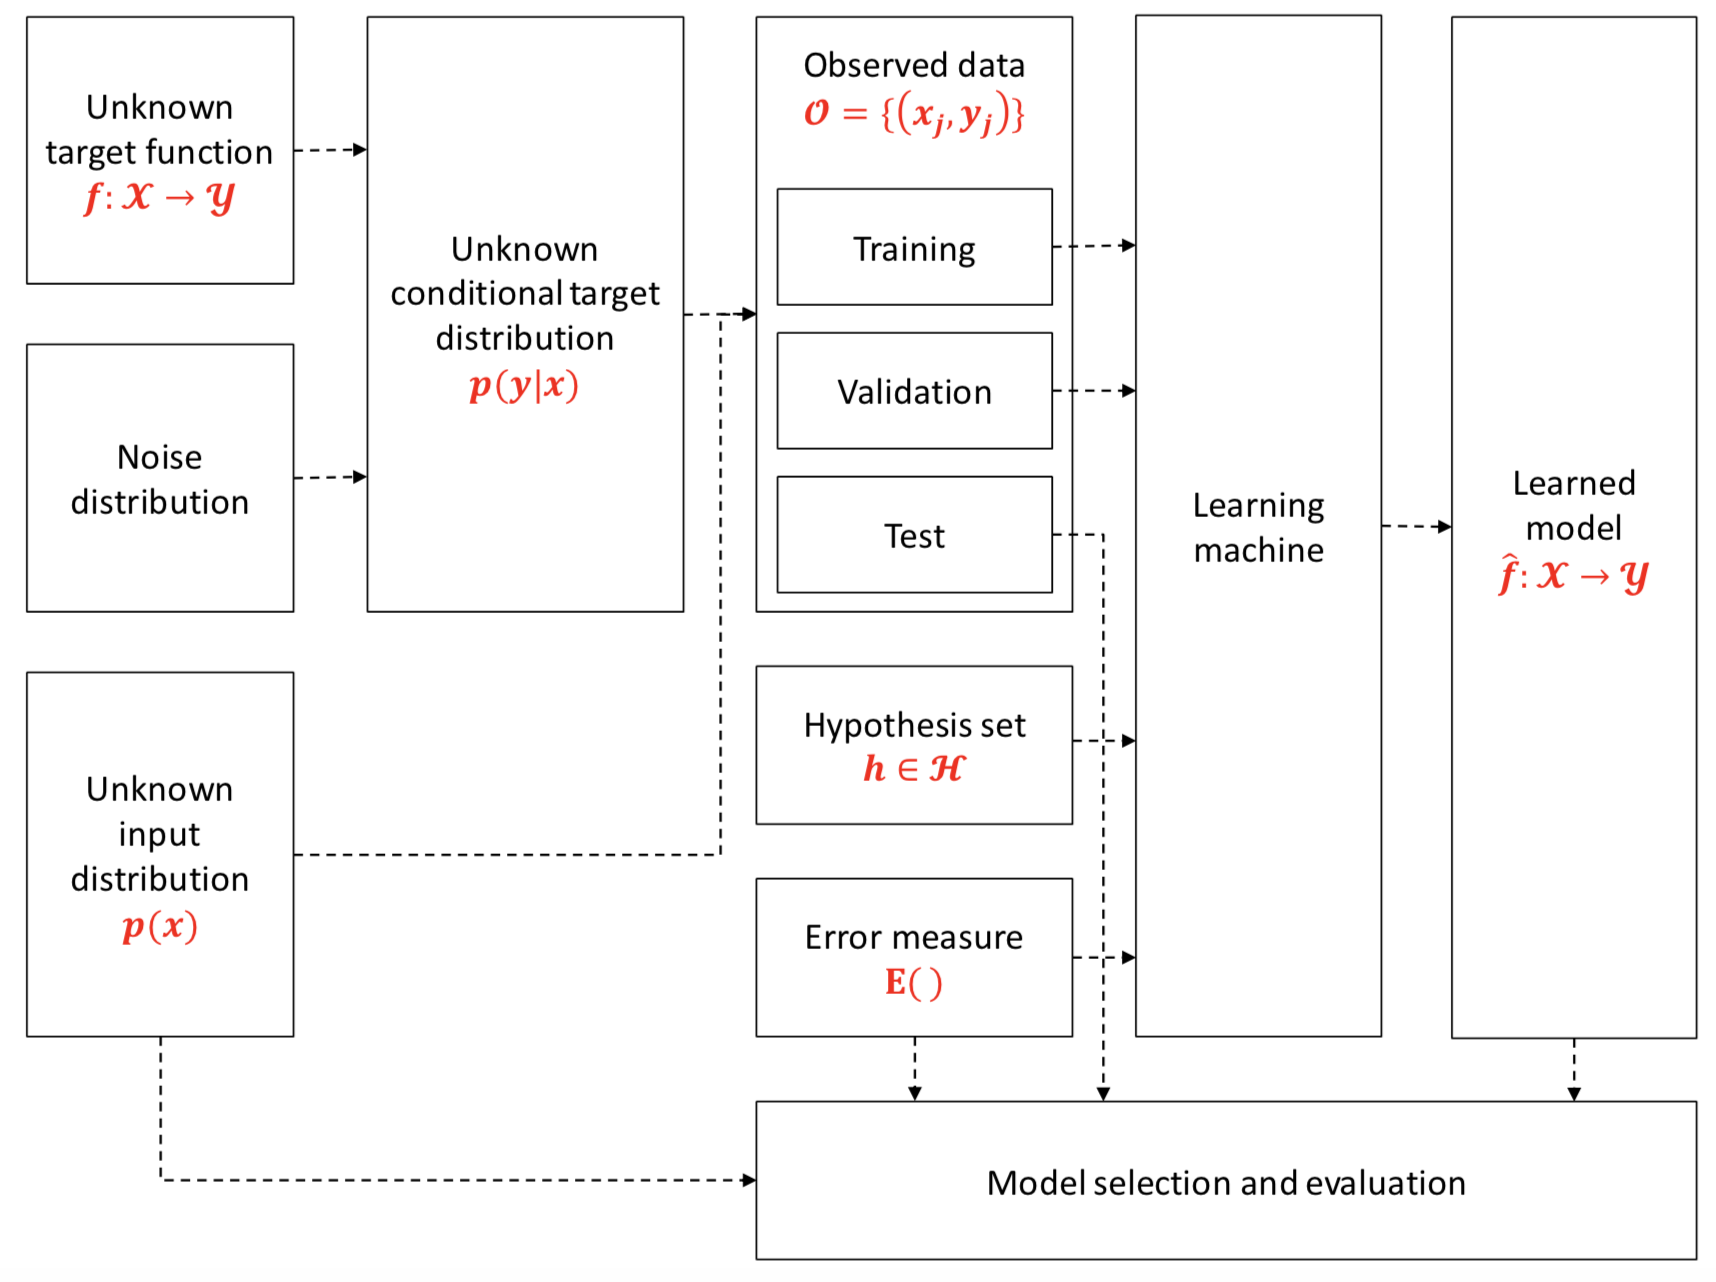
\includegraphics[width=0.5\textwidth]{figures/chapter_6_supervised_learning_overview.png}
		\caption{Overview of supervised learning framework}
		\label{fig:chapter_6_supervised_learning}
	\end{figure}
	\item Discussion of error measuring
	\begin{itemize}
		\item \textit{Risk} $E(h,f)$ describes the distance between our hypothesis $h$ and the target function $f$
		\item \textit{Loss} is the point-wise risk $e(h(x),f(x))$
		\item Given the evidence $p(x)$, we can determine the risk by $E(h,f)=\int e(h(x), f(x)) p(x) dx$
		\item However, this integral can (usually) not be computed, and only approximated by Monte-Carlo integration. 
		\item For definitions of $e$, we can use metrics like F1 or accuracy (classification), or MSE etc. (regression)
		\item The in-sample error is the average loss over all training points $E_{in}(h)=\frac{1}{N}\sum_{(x,y) \in \mathcal{O}_{\text{train}}} e(y, h(x))$
		\item The out-of-sample error accordingly for points not in the training set:\\
		$E_{out}(h)=\int_{\mathcal{X}\setminus \mathcal{O}_{\text{train}}} e(h(x), f(x)) p(x) dx$
	\end{itemize}
	\item We select the model with the lowest in-sample error, but need to be careful with overfitting
\end{itemize}
\subsection{PAC Learnability and VC dimensionality}
\begin{itemize}
	\item ``Probably approximately correct learning''
	% \item A hypothesis set is PAC learnable if a learning algorithm exists that can minimize the generalization error to $|E_{out}(\hat{f}) - E_{in}(\hat{f})| < \epsilon$ with a probability of $1-\delta$
	\item A hypothesis set is PAC learnable when it can be shown that given any value of $\delta$, $\epsilon$ there is an $N$ (number of samples) where with probability $1-\delta$ the difference between the in-sample and out-of-sample error is less than $\epsilon$. 
	\item \textit{Probably}: $1-\delta$, \textit{Approximate correct}: $|E_{out}(\hat{f}) - E_{in}(\hat{f})| < \epsilon$ 
	\item For a finite set of $M$ hypotheses, we determine it by:
	$$E_{out}(\hat{f}) \leq E_{in}(\hat{f}) + \sqrt{\frac{1}{2N}\log \frac{2M}{\delta}}$$
	Hence, every finite set of hypotheses is PAC learnable, and we can calculate the expected error given number of samples $N$, hypothesis set size $M$, and probability $\delta$
	\item For infinite set of hypotheses, we can look at VC dimensionality
	\begin{itemize}
		\item We say that a set of input vectors $X$ is shattered by a hypothesis set $\mathcal{H}$ if it can represent all possible labeling
		\item The VC dimension of $\mathcal{H}$ is an $X$ with the highest cardinality $D$. Note that not all possible point sets of cardinality $D$ must be shattered by $\mathcal{H}$. It is sufficient if it is true for at least one. 
		\item Example for a perceptron:
		\begin{figure}[ht!]
			\centering
			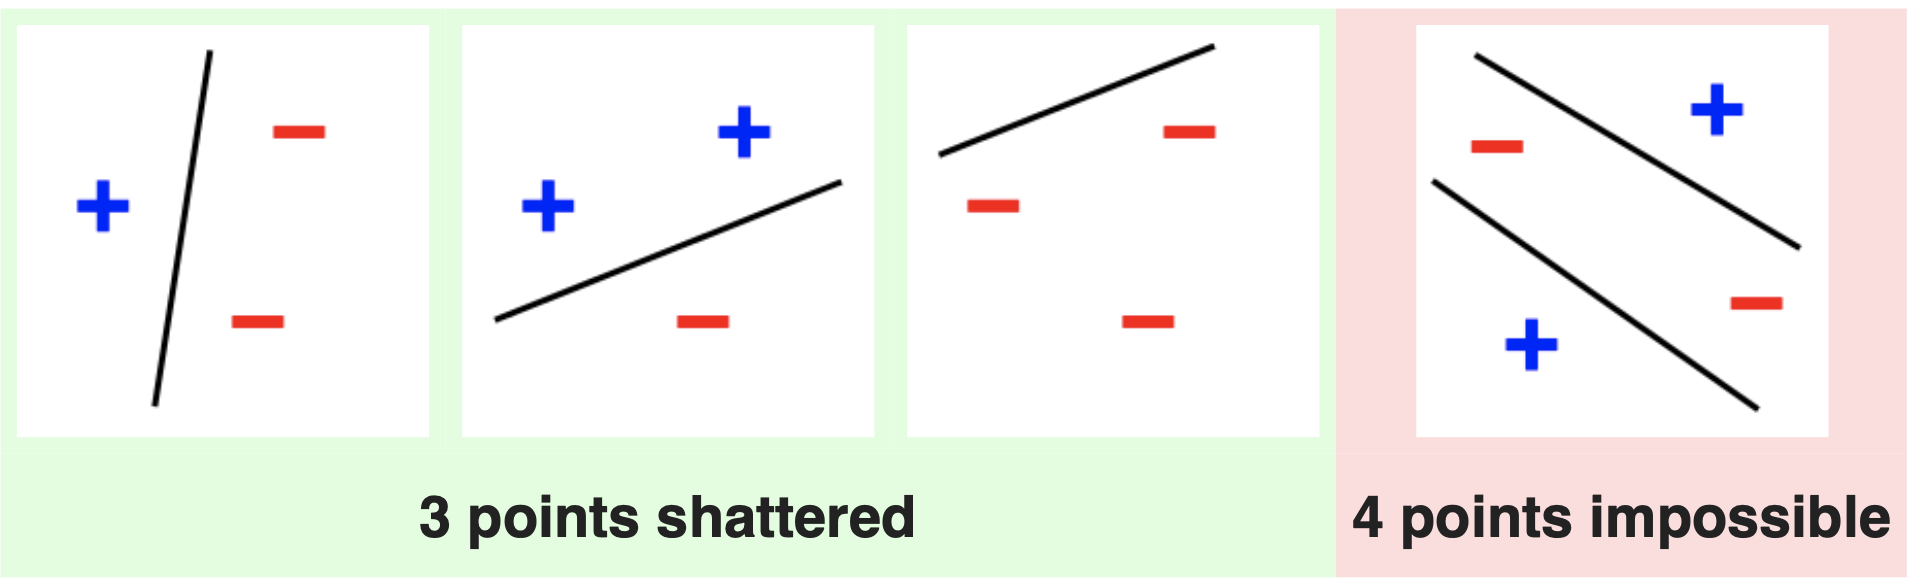
\includegraphics[width=0.3\textwidth]{figures/chapter_6_VC_dimensions.png}
		\end{figure}
	
		The VC dimension of a perceptron in 2 dimensions is $3$, because there exists no set of 4 points that can be shattered (i.e. for which we can learn any labeling)
		\item If the hypothesis set can represent any labeling for an arbitrary large set $X$, it has a VC dimension of $\infty$
		\item Important finding: all hypothesis set with a finite VC-dimension are PAC learnable
		\item We can 
	\end{itemize}
	\item Some implications from this study
	\begin{itemize}
		\item Given a few training samples, it is easy to get a low in-sample error. But with increasing number of samples, the out-of-sample error decreases
		\item In addition, for a fixed $N$, we can study the influence of more complex hypotheses and find the best compromise
		\item  
	\end{itemize}
\end{itemize}